\documentclass[main.tex]{subfiles}
\begin{document}

\section{Indivisibility of the photon}

\subsection{Background}

The fact that light is made up of indivisible photons is not the only possible explanation for the photoelectric effect \cite[]{thornObservingQuantumBehavior2004}: it can also be described with a quantized surface and a classical electromagnetic field. 

So, we need an experiment to unambiguously show that light is indeed made up of indivisible \emph{quanta}.

\subsection{Description of the apparatus}

\begin{figure}[ht]
\centering


\tikzset{every picture/.style={line width=0.75pt}} %set default line width to 0.75pt        

\begin{tikzpicture}[x=0.75pt,y=0.75pt,yscale=-1,xscale=1]
%uncomment if require: \path (0,300); %set diagram left start at 0, and has height of 300

%Shape: Rectangle [id:dp3902522124544314] 
\draw   (37,72) -- (111.5,72) -- (111.5,112) -- (37,112) -- cycle ;
%Shape: Wave [id:dp29533096809256154] 
\draw  [dash pattern={on 4.5pt off 4.5pt}] (112,93) .. controls (116.08,95.56) and (119.98,98) .. (124.5,98) .. controls (129.02,98) and (132.92,95.56) .. (137,93) .. controls (141.08,90.44) and (144.98,88) .. (149.5,88) .. controls (154.02,88) and (157.92,90.44) .. (162,93) .. controls (166.08,95.56) and (169.98,98) .. (174.5,98) .. controls (179.02,98) and (182.92,95.56) .. (187,93) .. controls (191.08,90.44) and (194.98,88) .. (199.5,88) .. controls (204.02,88) and (207.92,90.44) .. (212,93) .. controls (216.08,95.56) and (219.98,98) .. (224.5,98) .. controls (229.02,98) and (232.92,95.56) .. (237,93) .. controls (237.17,92.9) and (237.33,92.79) .. (237.5,92.69) ;
%Shape: Rectangle [id:dp5615185733257464] 
\draw   (238,73) -- (308,73) -- (308,113) -- (238,113) -- cycle ;
%Shape: Chord [id:dp5426551407812648] 
\draw   (307.1,184.93) .. controls (308.92,188.52) and (309.95,192.47) .. (310,196.63) .. controls (310.17,213.2) and (294.64,226.8) .. (275.31,227) .. controls (255.99,227.2) and (240.18,213.93) .. (240,197.37) .. controls (239.96,193.2) and (240.91,189.23) .. (242.65,185.61) -- cycle ;
%Shape: Wave [id:dp5480038928028264] 
\draw  [dash pattern={on 4.5pt off 4.5pt}] (309,91) .. controls (313.08,93.56) and (316.98,96) .. (321.5,96) .. controls (326.02,96) and (329.92,93.56) .. (334,91) .. controls (338.08,88.44) and (341.98,86) .. (346.5,86) .. controls (351.02,86) and (354.92,88.44) .. (359,91) .. controls (363.08,93.56) and (366.98,96) .. (371.5,96) .. controls (376.02,96) and (379.92,93.56) .. (384,91) .. controls (388.08,88.44) and (391.98,86) .. (396.5,86) .. controls (401.02,86) and (404.92,88.44) .. (409,91) .. controls (413.08,93.56) and (416.98,96) .. (421.5,96) .. controls (426.02,96) and (429.92,93.56) .. (434,91) .. controls (434.17,90.9) and (434.33,90.79) .. (434.5,90.69) ;
%Shape: Square [id:dp4933988712132191] 
\draw   (435,69) -- (485,69) -- (485,119) -- (435,119) -- cycle ;
%Straight Lines [id:da6356953181395324] 
\draw    (435,69) -- (485,119) ;
%Shape: Wave [id:dp43746939652005445] 
\draw  [dash pattern={on 4.5pt off 4.5pt}] (274.13,112.25) .. controls (271.88,116.33) and (269.75,120.23) .. (269.75,124.75) .. controls (269.75,129.27) and (271.88,133.17) .. (274.13,137.25) .. controls (276.37,141.33) and (278.5,145.23) .. (278.5,149.75) .. controls (278.5,154.27) and (276.37,158.17) .. (274.13,162.25) .. controls (271.88,166.33) and (269.75,170.23) .. (269.75,174.75) .. controls (269.75,178.44) and (271.17,181.71) .. (272.9,185) ;
%Shape: Wave [id:dp8229982636223081] 
\draw  [dash pattern={on 4.5pt off 4.5pt}] (460.13,120.25) .. controls (457.88,124.33) and (455.75,128.23) .. (455.75,132.75) .. controls (455.75,137.27) and (457.88,141.17) .. (460.13,145.25) .. controls (462.37,149.33) and (464.5,153.23) .. (464.5,157.75) .. controls (464.5,162.27) and (462.37,166.17) .. (460.13,170.25) .. controls (457.88,174.33) and (455.75,178.23) .. (455.75,182.75) .. controls (455.75,186.44) and (457.17,189.71) .. (458.9,193) ;
%Shape: Chord [id:dp06188698806334458] 
\draw   (494.22,193.27) .. controls (496.01,196.87) and (497,200.84) .. (497,205) .. controls (497,221.57) and (481.33,235) .. (462,235) .. controls (442.67,235) and (427,221.57) .. (427,205) .. controls (427,200.84) and (427.99,196.87) .. (429.78,193.27) -- cycle ;
%Shape: Wave [id:dp9566458935440425] 
\draw  [dash pattern={on 4.5pt off 4.5pt}] (484.75,91.63) .. controls (488.83,93.87) and (492.73,96) .. (497.25,96) .. controls (501.77,96) and (505.67,93.87) .. (509.75,91.63) .. controls (513.83,89.38) and (517.73,87.25) .. (522.25,87.25) .. controls (526.77,87.25) and (530.67,89.38) .. (534.75,91.63) .. controls (538.83,93.87) and (542.73,96) .. (547.25,96) .. controls (550.94,96) and (554.21,94.58) .. (557.5,92.85) ;
%Shape: Chord [id:dp22990401692182982] 
\draw   (557.27,60.78) .. controls (560.87,58.99) and (564.84,58) .. (569,58) .. controls (585.57,58) and (599,73.67) .. (599,93) .. controls (599,112.33) and (585.57,128) .. (569,128) .. controls (564.84,128) and (560.87,127.01) .. (557.27,125.22) -- cycle ;

% Text Node
\draw (48,84) node [anchor=north west][inner sep=0.75pt]   [align=left] {LASER};
% Text Node
\draw (253,85) node [anchor=north west][inner sep=0.75pt]   [align=left] {SPDC};
% Text Node
\draw (256,193) node [anchor=north west][inner sep=0.75pt]   [align=left] {Gate};
% Text Node
\draw (452,204) node [anchor=north west][inner sep=0.75pt]   [align=left] {R};
% Text Node
\draw (569,83) node [anchor=north west][inner sep=0.75pt]   [align=left] {T\\};
% Text Node
\draw (450,32) node [anchor=north west][inner sep=0.75pt]   [align=left] {BS};


\end{tikzpicture}
\caption{Indivisibility experiment setup.}
\label{fig:spdc}
\end{figure}

A schematic for the apparatus is provided in figure \ref{fig:spdc}. 
A LASER produces a coherent beam of light, whose photons have energy \(2 \hbar \omega  \). This beam impacts upon a nonlinear crystal, where a photon each \(\num{e6} \divisionsymbol \num{e8}\) undergoes Spontaneous Parametric Down-Conversion, being split into two entangled photons, each with energy \(\hbar \omega \). 
These are emitted in two cones which intersect along two rays. 

Along one of these the photon is sent to a detector called ``Gate'', along the other the photon is sent towards a beamsplitter; from this it can go to either of two detectors, which are called ``T'' and ``R'' for ``Transmitted'' and ``Reflected''.

Each detector has a nonzero ``dark count'' --- clicks in the absence of a photon ---, and an efficiency different from \SI{100}{\percent}. Also, photons might be absorbed by the air in their path or by the beamsplitter.

Let us first consider the problem ideally, in the absence of these sources of error.
Then, a click in the ``Gate'' detector signals that a photon is also coming through the beamsplitter. 

Then, according to quantum theory if that photon is reflected it is not transmitted, and vice versa. 
If, instead, we describe the electromagnetic field classically we expect the detection probability per unit time for both ``R'' and ``T'' to be proportional to the incoming power, with no correlation nor anticorrelation between them. 

We may quantify this by introducing the second coherence parameter 
%
\begin{align}
g^{(2)} = \frac{ \mathbb{P} (RT | G) }{\mathbb{P}(R|G) \mathbb{P}(T|G)}
\,,
\end{align}
%
where by \(RT | G\) we mean the event of observing a R+T coincidence, conditioned upon seeing a click by the gate; the notation for the other ones is similar. 

This can be computed by counting the number of coincidences, the expression is 
%
\begin{align}
g^{(2)}_{\text{measured}} = \frac{N_{TRG} N_G}{N_{RG} N_{TG}}
\,.
\end{align}

This parameter allows us to quantify the correlation or anticorrelation between the detectors: let us consider some simple cases. 

\begin{enumerate}
    \item In quantum theory, we expect \(\mathbb{P}(RT|G) = 0\), since the photon cannot be detected at both sides --- therefore \(g^{(2)} = 0\).
    \item In classical theory, we expect \(\mathbb{P}(RT|G) = \mathbb{P}(R|G) \mathbb{P}(T|G)\), since the events are independent, at each moment in time. If the laser's intensity is constant this can be extrapolated through the whole observation to yield \(g^{(2)} = 1\). 
    \item In classical theory we can also consider the effect of a time-varying intensity. In that case, this intensity \(I(t)\) is split into \(\mathcal{T}I(t)\) and \(\mathcal{R}I(t)\) at the detector, where \(\mathcal{T}\) and \(\mathcal{R}\) are the transmission and reflection coefficients, satisfying \(\mathcal{T} + \mathcal{R} =1\). Then, we get 
    %
    \begin{align}
    g^{(2)} = \frac{ \int \mathcal{T} I(t) \mathcal{R}I(t) \dd{t}}{ \int \mathcal{T} I(t) \dd{t} \int \mathcal{R} I(t) \dd{t}} \geq 1
    \,,
    \end{align}
    %
    by the Cauchy-Schwarz inequality. All the temporal integrals are definite ones, the bounds corresponding to the time of observation. For a small enough temporal variation of the intensity, the result approaches 1. 
\end{enumerate}

This is all in the case of an ideal detector, with no losses nor dark count. We do not explore the effect of these theoretically; instead in the data analysis these effects were parametrized and simulated as stochastic variables. 

\subsection{Data preparation}

The output of the timetagger is a table of times and corresponding channel values.
Each entry of this table represents a photon detection at a single detector.
The times are expressed as integer multiples of the temporal resolution of the timetagger, which is nominally \SI{80.955}{ps}.

There is a slight complication: the timetagger exhibits a slight preference for odd values of the integer which represents the time, as opposed to even ones. This effect does not pose an issue for our analysis, as long as we bin our arrival times in time intervals of \(2 \times \SI{80.955}{ps}\). 

We want to calculate \textbf{coincidences}. The temporal resolution we have corresponds to a length scale of around \SI{5}{cm}, which is smaller than the size of the apparatus, so we are able to see systematic time differences between the arrival times corresponding to the light's travel time. 

In figure \ref{fig:single_photon_timedifferences} we plot the differences between the arrival times of photons to either R or T and the gate. 

\begin{figure}[ht]
\centering
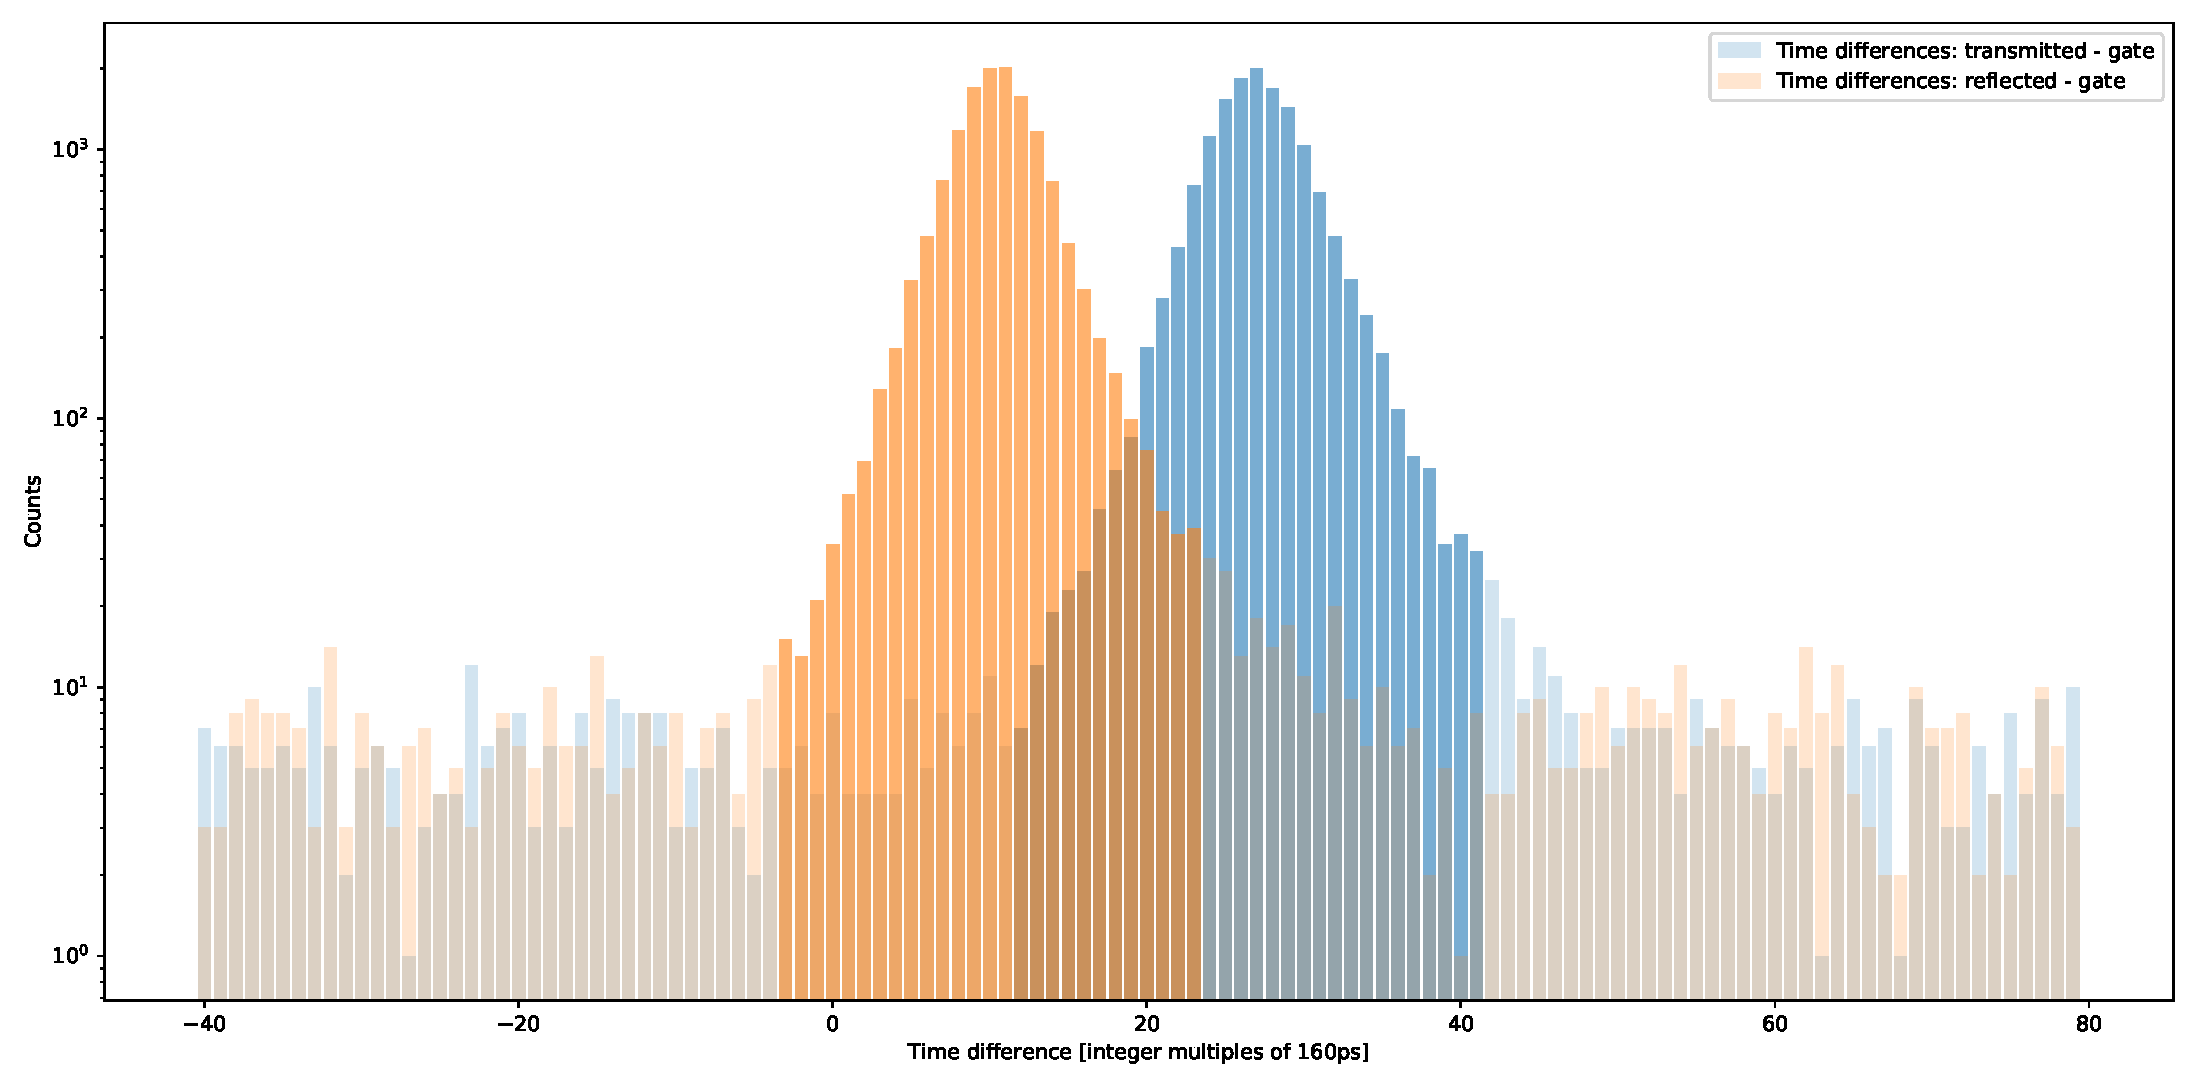
\includegraphics[width=\textwidth]{figures/single_photon_timedifferences}
\caption{Time differences. In a darker colour the events which were counted as coincidences are shown.}
\label{fig:single_photon_timedifferences}
\end{figure}

We see distinct Gaussian peaks a few nanoseconds away from zero. We fit these, and find the means to be 10 and 27 respectively, while the standard deviations are both 3.

Outside of these peaks, there is a constant noise background of the order of 10 detections per \(\Delta t\) bin.
We choose to consider as coincidences events which lie within 5 standard deviations in each peak, since around that point the values become compatible with those of the background.

This allows us to compute \(N_{RG}\) and \(N_{TG}\); \(N_G\) is simply the total count of the gate; for \(N_{TRG}\) we count a coincidence if we have a coincidence on both R and T corresponding to the \emph{same} gate tick. 

This procedure yields \(N_G = 1554341\), \(N_{TG}=14829\), \(N_{RG}=13870\), \(N_{TRG}=2\).
Therefore, we compute the preliminary result:
%
\begin{align}
g^{(2)} \approx \num{.015}
\,.
\end{align}

\subsection{Simulation}

In order to perform a proper Bayesian analysis of these results, we need to compute the Bayes Factor in: 
%
\begin{align}
\frac{\mathbb{P}(\text{quantum} | \text{data})}{\mathbb{P}(\text{classical} | \text{data})}
= \underbrace{\frac{\mathbb{P}(\text{data} | \text{quantum})}{\mathbb{P}(\text{data} | \text{classical})}}_{\text{Bayes Factor}}
\frac{\mathbb{P}(\text{quantum})}{\mathbb{P}(\text{classical})}
\,.
\end{align}

Some clarifications are in order. By ``data'' we mean the tuple \((N_G, N_{TG}, N_{RG}, N_{TRG})\). I use the notation \(\mathbb{P}\) for ease of reading, but the Bayes Factor is really a ratio of two probability \emph{densities}.\footnote{Or rather, since the detection numbers are so large, it is convenient to model them as continuous.}
The two models --- quantum and classical --- are simulated as follows.

\begin{enumerate}
    \item The number \(N_G\) is fixed as the total number of potential event detections for either detector. 
    \item We set two parameters: \(r\), the detection rate, and \(e\), the error rate.
    Each detector is assumed to detect a fraction \(r\) of the incoming photons, and to make an error a fraction \(e\) of the time --- this can be either a dark count, or a missed detection (although since \(r \ll 1\), it mostly accounts for the former).\footnote{A small correction is needed to account for the detector asymmetry. We observe \(N_{TG} - N_{RG} \approx 1000\), which is on the order of \(10 \sigma \) using Poisson statistics: so, there is a bias in the detectors. This is accounted for by extracting the factor \(N_{TG} / N_{RG}\) from the data and applying it as a \emph{constant bias} for each simulated ratio between the detectors, for both models.}
    \item In the classical case, the detectors are simulated independently, while in the quantum case a ``which-way'' parameter is simulated with a \(1/2\) chance for either direction, and only the selected detector may see the photon. In order to account for the halving of the number of photons seen globally (and to compare the numbers for the classical and quantum case directly), the detection rate for the classical is halved.
    \item The computation for \(\mathbb{P}(\text{data} | M)\) where \(M\) is a model is as follows: 
    %
    \begin{align}
    \mathbb{P}(\text{data} | M) = 
    \int \mathbb{P}(\text{data} | M; r, e) f(r) f(e) \dd{r} \dd{e}
    \,,
    \end{align}
    %
    where \(f(r)\) and \(f(e)\) are the prior probability distributions for the detection rate and the error rate. 
    Both of these were chosen to be uniform, and their ranges were not constrained \emph{a priori} to be smaller than \([0,1]\); however after exploratory runs it was found that the likelihoods for both models were nonzero only in a certain region, so only those were simulated for computational efficiency.
    
    The definitive intervals were \(r \in [\num{.012}, \num{0.019}]\) and \(e \in [\num{3.0e-7}, \num{1.8e-2}]\); 50 points were simulated for each, they were linearly spaced for \(r\) and logarithmically spaced for \(e\). 
    \item For each pair of parameters, \(N_G\) photons were simulated for \(N _{\text{sim}}\) times. In the final run, we set \(N _{\text{sim}}\) to 600. 
    
    For each of the \(N _{\text{sim}}\) simulations the values \(N_{TG}\), \(N_{RG}\) and \(N_{TRG}\) are extracted (also, trivially, the fixed value of \(N_G\)). 
    From these, a gaussian Kernel-Density Estimation technique (using Scott's rule \cite[]{scipycontributorsScipyStatsGaussian2019,scottMultivariateDensityEstimation2015}) is used to estimate the value of the multivariate PDF at the point corresponding to the measured data for both models: the likelihood of the data.
    The variation of these likelihoods is shown in figure \ref{fig:both_logpdfs}. 
    \item These likelihoods are integrated along \(r\) and \(e\) to yield a total value. We find 
    %
    \begin{align}
    BF = \frac{\mathbb{P}(\text{data} | \text{quantum})}{\mathbb{P}(\text{data} | \text{classical})}
    \approx \num{e77}
    \,.
    \end{align}
\end{enumerate}

\begin{figure}[ht]
\centering
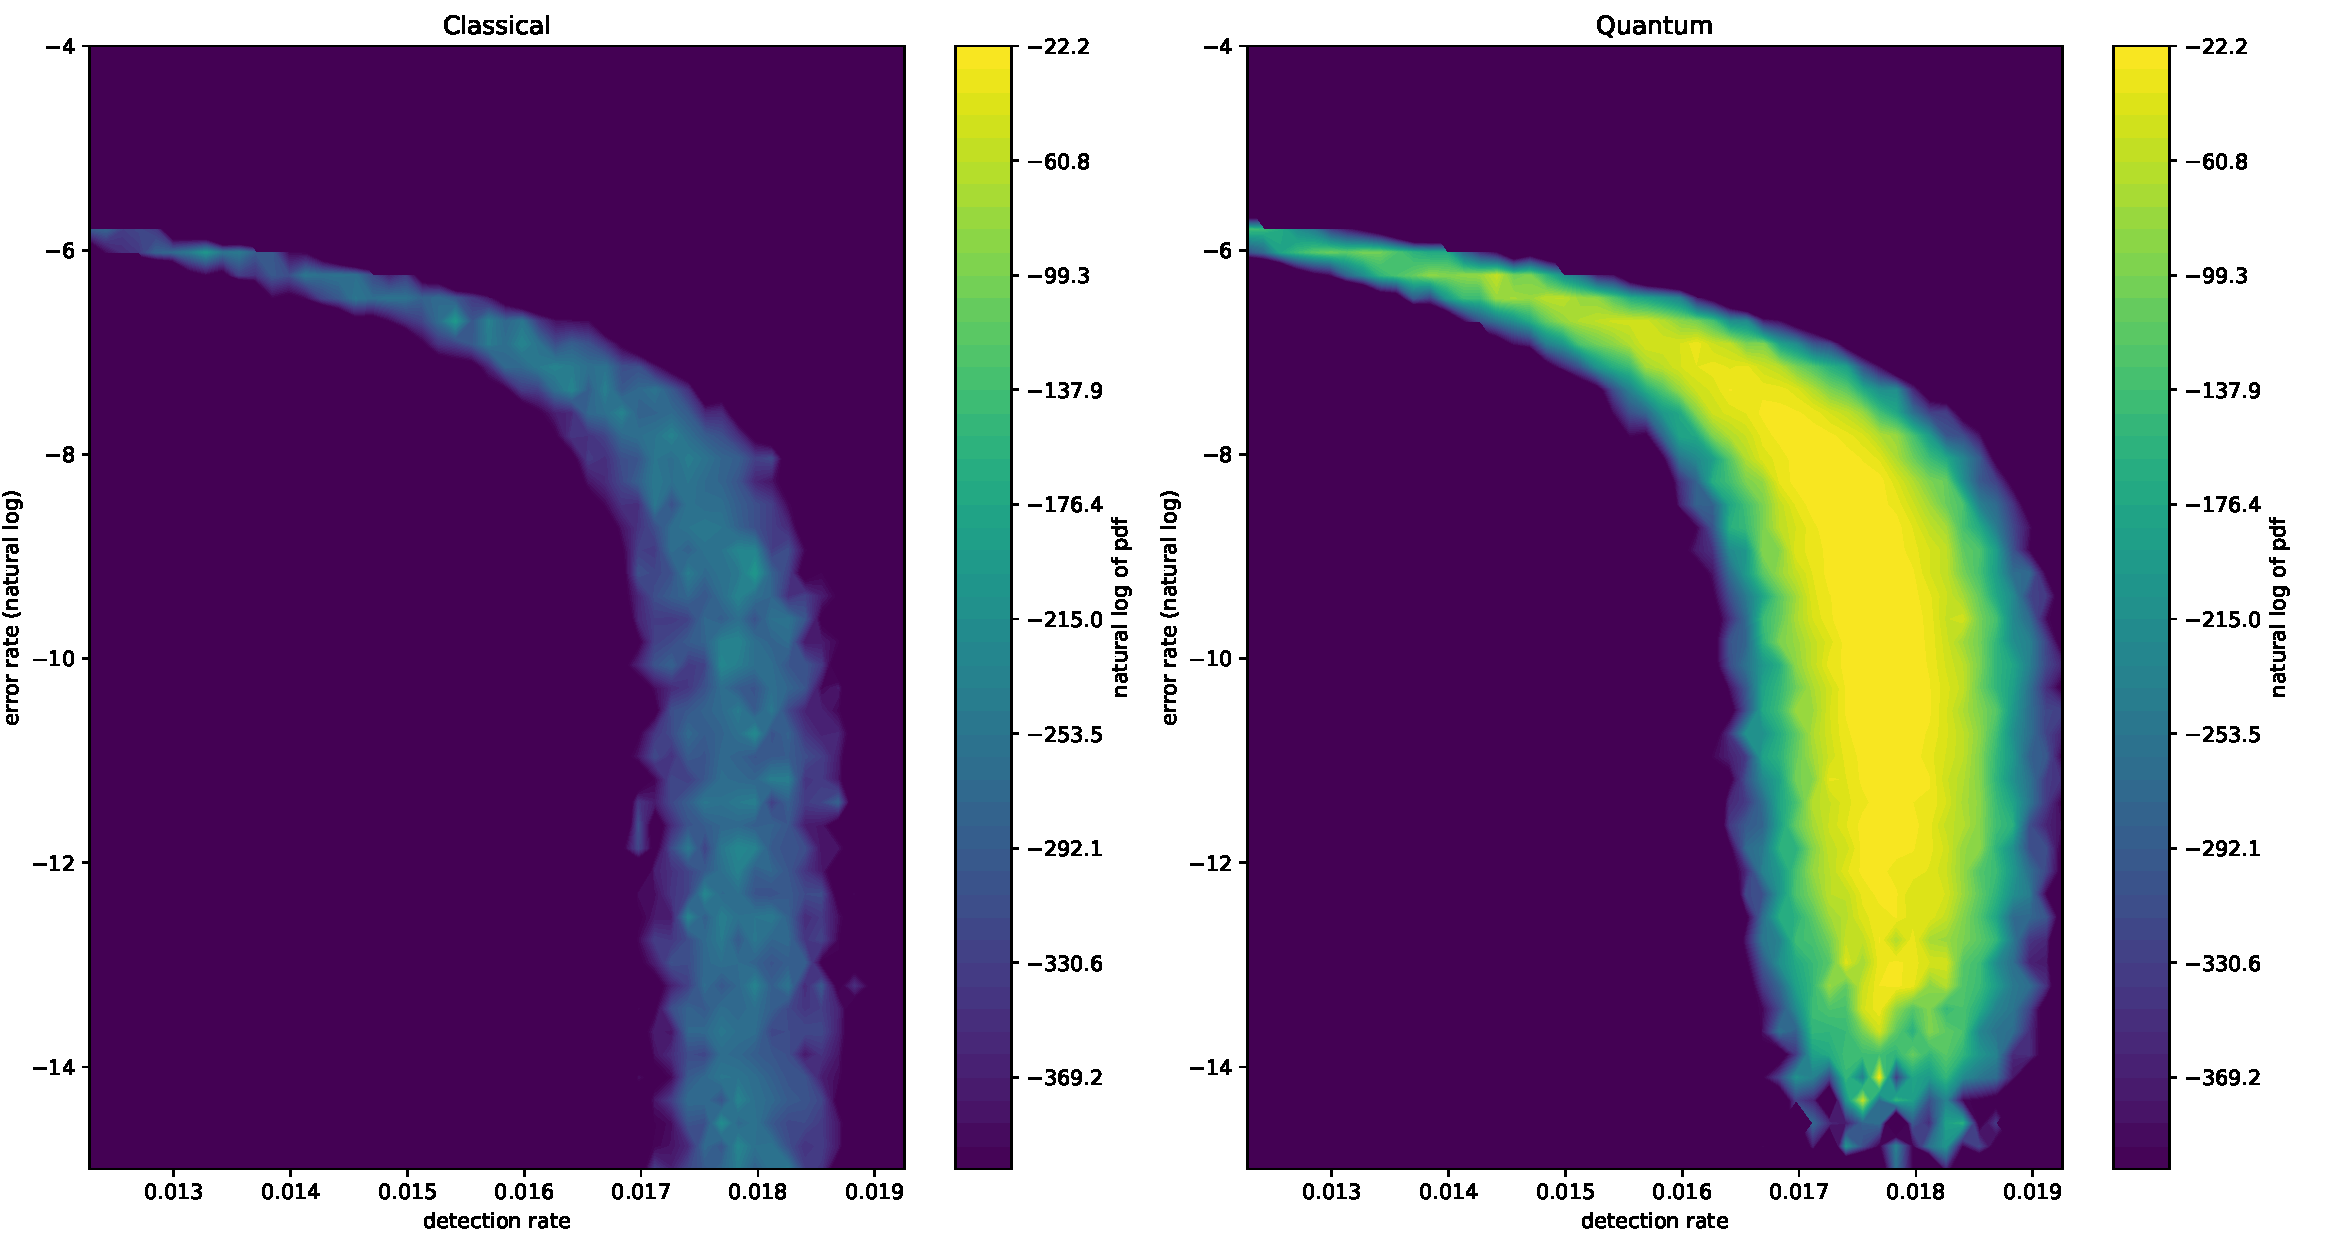
\includegraphics[width=\textwidth]{figures/both_logpdfs}
\caption{Log-PDFs for the classical and quantum cases. Note the log-scale of the colours: the likelihood of the classical model is \emph{heavily} suppressed compared to the one of the quantum model.}
\label{fig:both_logpdfs}
\end{figure}

The code which performs these simulations can be found at \url{https://github.com/jacopok/quantum_optics/tree/master/single_photon}. 

\end{document}
